\documentclass[serif, final, noamsthm]{beamer} %
\usepackage{enumitem}
\usepackage{algorithm2e}
%\bibliographystyle{plain}

\mode<presentation>{\usetheme{YNCTheme}}
\usepackage[T1]{fontenc}
\usepackage[utf8]{inputenc}
\usepackage{amsmath, amssymb, latexsym, graphicx}
\usepackage[orientation=landscape,size=a0,scale=1.3]{beamerposter}
\usepackage{array,booktabs,tabularx, ragged2e}
\newcolumntype{Z}{>{\centering\arraybackslash}X} 
\newcommand{\pphantom}{\textcolor{white}}
%\listfiles
\usepackage{biblatex}
\addbibresource{references.bib}

\newtheorem{thm}{Theorem}
\newtheorem{lem}[thm]{Lemma}
\newtheorem{sublem}[thm]{Sublemma}
\newtheorem{prop}[thm]{Proposition}
\newtheorem{cor}[thm]{Corollary}
\newtheorem{conc}[thm]{Conclusion}
\newtheorem{conj}[thm]{Conjecture}
%\theoremstyle{definition}
\newtheorem{defn}[thm]{Definition}
\newtheorem{cond}[thm]{Condition}
\newtheorem{asm}[thm]{Assumption}
\newtheorem{ntn}[thm]{Notation}
\newtheorem{prob}[thm]{Problem}
%\theoremstyle{remark}
\newtheorem{rmk}[thm]{Remark}
\newtheorem{eg}[thm]{Example}
%\newtheorem*{hint}{Hint}

\newlength{\columnheight}
\setlength{\columnheight}{.78\textheight}

\newcommand{\refPaper}[1]{[\ref{itm:#1}]}
\newcommand{\startPoster}{
	\begin{frame}
	\begin{columns}[t]
}

\newcommand{\finishPoster}{
\end{columns}
\end{frame}
}

\newcommand{\newColumn}[2]{
	\begin{column}{#1}
	\begin{beamercolorbox}[center,wd=\textwidth]{postercolumn}
	\begin{minipage}[T]{\textwidth} %.95
	\parbox[t][\columnheight]{\textwidth}{ 
	#2
	}\end{minipage}
	\end{beamercolorbox}
	\end{column}
}

\newenvironment{proof}[1][Proof.]{\begin{trivlist}
\item[\hskip \labelsep {\bfseries #1}]}{\end{trivlist}}
\AtEndEnvironment{proof}{\null\hfill\blacksquare}%

\setenumerate[1]{%
  label=\protect\usebeamerfont{enumerate item}%
        \protect\usebeamercolor[fg]{enumerate item}%
        \insertenumlabel.}
\newcommand{\myEmail}{Your Email@seattleu.edu}
%\newcommand{\conferenceName}{Type the Title of the Conference Here?  Or maybe some other info?}

%%%%%%%%%%%%%%%%%%%%%%%%%%%%%%%%%%%%%%%%%%%%%%%%%%%%%%%%%%%%%%%%%%%%%%%%%%%%%%%%%%%%%%%

 
\title{Algorithmic Construction of an Adjoint of an Ordinary Differential Operator in Julia}
\author{Sultan Aitzhan $\mid$ Email: a.sultan@u.yale-nus.edu.sg}
% = = = = = = = = = = = = = = = = = = = = = = = = = = = = = = = = = = = = = = = = = = = = =
\begin{document}
\begin{center}
\begin{frame}
\begin{columns}[t]
% = = = = = = = = = = = = = = = = = = = = = = = = = = = = = = = = = = = = = = = = = = = = =
% First Column
% = = = = = = = = = = = = = = = = = = = = = = = = = = = = = = = = = = = = = = = = = = = = =
\newColumn{.31\textwidth}{

\begin{block}{Abstract}
\justifying  
Given an operator, its adjoint is a linear transformation that can be used to characterise a wide range of phenomena in mathematics and physics. In this project we seek to characterise an adjoint of an ordinary differential operator with multipoint homogeneous conditions. Extending the ideas of Linfan Xiao, we show that the operator and its adjoint satisfy the multipoint form formula. In doing so, we provide an explicit construction of adjoint multipoint conditions, and provide an explicit checking test to determine whether a given set of multipoint conditions satisfies the adjoint equation. Finally, we implement a method of deriving the adjoint multipoint conditions in programming language julia, thus providing a fast way to compute the adjoint.
\end{block}

\begin{block}{Multipoint Conditions}
\justifying
Consider an interval $[0,1],$ and suppose that we want specify the behaviour of $q(x)$ on this interval not just at the endpoints but also at finitely many points in the interior. Then, we can represent one such specification by an expression
\[ \alpha_{ijl} q_l^{(j)}(x_{l-1}) + \beta_{ijl} q_l^{(j)}(x_{l}), \]
where $x_{l-1}, x_l$ are two adjacent points, $q_l$ is the function $q$ but restricted to the interval $(x_{l-1}, x_l),$ and $q_l^{(j)}$ is the $j^{\text{th}}$ derivative of $q_l.$ Combining all such specifications yields an expression of the form
\begin{equation*}
\sum^{k}_{l=1} \sum^{n-1}_{j=0}[\alpha_{jl} q_l^{(j)}(x_{l-1}) + \beta_{jl} q_l^{(j)}(x_{l})]
\end{equation*}
which we call a \textbf{multipoint form}. Then, requiring that a multipoint form be equal to some number, and combining these equations yileds one vector equation, which we term as a \textbf{multipoint condition}. The image below provides an intuitive idea of the multipoint conditions. 
\vskip2ex
\begin{center}\includegraphics[width=0.7\textwidth]{figures/BC-MC-NC-010.mps}\end{center}
\end{block}
\begin{block}{Formulation of the Problem}
Consider a closed interval $[a,b].$ Fix $n\in\mathbb{N},$ and let the differential operator be defined as
\begin{equation}\label{operatorL}
L  := \sum^n_{k=0} a_k(x)\left( \frac{d}{dx}\right)^k, \mbox{ where } a_k(x) \in C^{\infty}[a,b] \mbox{ and } a_n(x) \neq 0~ \forall x \in [a,b].
\end{equation} 
Fix $k \in \mathbb{N},$ and let $\{ a = x_0 < x_1 < \ldots < x_k = b\}$ be a partition of $[a,b].$ Consider a homogeneous multipoint value problem (MVP)
\[ \pi: Lq = 0, \qquad Uq = \vec{0},\]
where $U = (U_1, \ldots, U_m)$ is a vector multipoint form with 
\begin{equation}\label{MultipointConditions}
U_i(q) = \sum^{k}_{l=1} \sum^{n-1}_{j=0}[\alpha_{ijl} q_l^{(j)}(x_{l-1}) + \beta_{ijl} q_l^{(j)}(x_{l})], \qquad i \in \{ 1, \ldots, m \}, 
\end{equation}
where $\alpha_{ijl}, \beta_{ijl} \in \mathbb{R},$ and $q$ is sufficiently smooth. Our goal is to construct the adjoint multipoint value problem  to $\pi$
\[ 
\pi^+: L^+ q = 0, \qquad U^+q = \vec{0},
\] 
with 
\[ 
L^+  := \sum^n_{k=0} (-1)^k \left( \overline{a_k}(t) \frac{d}{dt}\right)^k,
\]
where $\overline{a_k}(t)$ is the complex conjugate of $a_k(t), ~ k = 0, \ldots, n,$ and $U^+$ is an appropriate vector multipoint form. Observe that for $\pi^+$ to be an adjoint problem to $\pi,$ we must have 
\[ \langle Lq, q \rangle = \langle q, L^+q\rangle. \]
\end{block}

% - - - - - - - - - - - - - - - - - - - - - - - - - - - - - - - - - - - - - - - - - - - - - - - - - - - - - - - - - - - - 
% - - - - - - - - - - - - - - - - - - - - - - - - - - - - - - - - - - - - - - - - - - - - - - - - - - - - - - - - - - - - 
}
%\begin{figure}
%\centering
%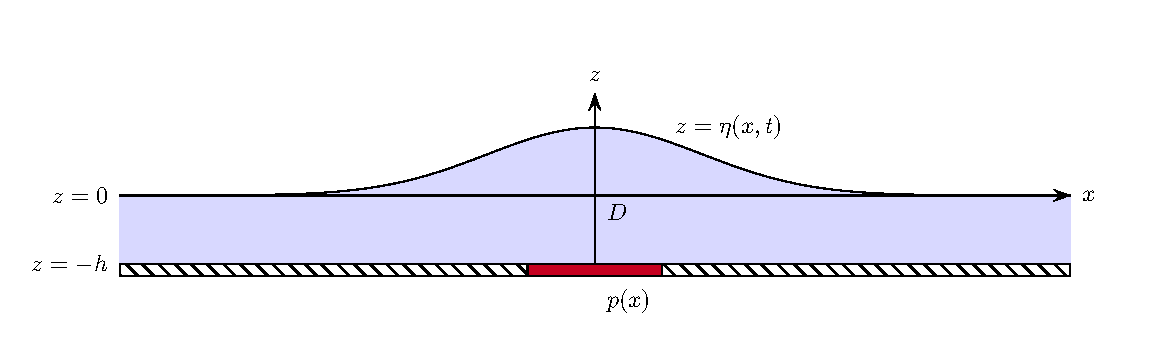
\includegraphics[width=.8\textwidth]{./figures/fluidDomain}
%\end{figure}

% = = = = = = = = = = = = = = = = = = = = = = = = = = = = = = = = = = = = = = = = = = = = =
% Second Column
% = = = = = = = = = = = = = = = = = = = = = = = = = = = = = = = = = = = = = = = = = = = = =

\newColumn{.31\textwidth}{	
\begin{block}{Multipoint Form Formula}
\begin{defn}
If $U = (U_1, \ldots, U_m)$ is any vector multipoint form with $\mathrm{rank}(U) = m,$ and $U_c = (U_{m+1}, \ldots, U_{2nk})$ is a vector multipoint form with $\mathrm{rank}(U_c) = 	2nk-m$ such that $\mathrm{rank}(U_{1}, \ldots, U_{2nk}) = 2nk,$ then $U$ and $U_c$ are \textbf{complementary vector multipoint forms}. 
\end{defn}

\begin{thm}[Multipoint Form Formula]\label{P2.BFF-theorem}
Given any vector multipoint form $U$ of rank $m,$ and any complementary vector form $U_c,$ there exist unique vector multipoint forms $U^+_c, U^+$ of rank $m$ and $2nk-m,$ respectively, such that
\begin{equation}\label{P2.BFF-eqn}
\sum_{l=1}^{k} [fg]_l(x_l) - [fg]_l(x_{l-1}) = Uf\cdot U^+_c g + U_c f \cdot U^+ g.
\end{equation}
\end{thm}
\end{block}

% - - - - - - - - - - - - - - - - - - - - - - - - - - - - - - - - - - - - - - - - - - - - - - - - - - - - - - - - - - - - 
% - - - - - - - - - - - - - - - - - - - - - - - - - - - - - - - - - - - - - - - - - - - - - - - - - - - - - - - - - - - - 
\begin{block}{Definition of the Adjoint}
Theorem \ref{P2.BFF-theorem} allows us to define an adjoint vector multipoint form. Namely, 

\begin{defn}
Suppose $U = (U_1, \ldots, U_m)$ is a vector multipoint form with $\mathrm{rank}(U) = m,$ along with the condition that $Uq = \vec{0}$ for functions $q$ sufficiently smooth. If $U^+$ is any vector multipoint form with  $\mathrm{rank}(U^+) = 2nk-m,$ determined as in Theorem \ref{P2.BFF-theorem}, then the equation 
\[ 
U^+q = \vec{0}
\]
is an \textbf{adjoint multipoint condition} to $Uq = \vec{0}.$
\end{defn}
In turn, the above lets us define the adjoint multipoint problem:

\begin{defn}
Suppose $U = (U_1, \ldots, U_m)$ is a vector multipoint form with $\mathrm{rank}(U) = m.$ Then, the problem of solving 
\[ \pi: Lq = 0, \qquad Uq = \vec{0},\] 
is called a homogeneous multipoint value problem. The problem of solving 
\[ \pi^+: L^+q = 0, \qquad U^+q = \vec{0},\] 
is an \textbf{adjoint multipoint value problem}. 
\end{defn}
The preceding construction allows us to state the following:

\begin{prop}
For $f,g$ sufficiently smooth, suppose $Uf = \vec{0}$ and $U^+g = \vec{0}.$ Then, $\langle Lf, g\rangle = \langle f, L^+g\rangle.$
\end{prop}

\begin{proof}
We apply the multipoint form formula \eqref{P2.BFF-eqn}
\begin{align*}
\langle Lf, g\rangle - \langle f, L^+g\rangle = Uf\cdot U^+_c g + U_c f \cdot U^+ g &= \vec{0}\cdot U^+_c g + U_c f \cdot \vec{0} = 0,
\end{align*} 
which completes the proof.
\end{proof}
\end{block}
          
	% - - - - - - - - - - - - - - - - - - - - - - - - - - - - - - - - - - - - - - - - - - - - - - - - - - - - - - - - - - - - 
         % - - - - - - - - - - - - - - - - - - - - - - - - - - - - - - - - - - - - - - - - - - - - - - - - - - - - - - - - - - - - 	
\begin{block}{Checking Adjointness}
\justifying
Note that for the appropriate matrices $M_l, N_l, P_l, Q_l,$ we can rewrite the multipoint conditions $Uf, U^+g$ as follows:
\begin{equation}\label{AdjointConditions}
Uf =
\sum^k_{l=1}
\begin{bmatrix}
M_l & N_l \\
\end{bmatrix} 
\begin{bmatrix}
\vec{f_l}(x_{l-1})  \\
\vec{f_l}(x_{l})
\end{bmatrix} \mbox{ and } 
U^+ g =
\sum^k_{l=1}
\begin{bmatrix}
P_l^* & Q_l^*
\end{bmatrix}
\begin{bmatrix}
\vec{g_l}(x_{l-1})  \\
\vec{g_l}(x_{l})
\end{bmatrix},
\end{equation}
where $\vec{f_l} = (f_l^{(0)}, f_l, \ldots, f_l^{(n-1)})$ is an $n \times 1$ column vector of derivatives.
The above notation allows to devise the following theorem.
\begin{thm}\label{P2.CA-theorem}
The boundary condition $U^+g = \vec{0}$ is adjoint to $Uf = \vec{0}$ if and only if \[ \sum^k_{l=1} M_lF^{-1}(x_{l-1})P_l = \sum^k_{l=1} N_l F^{-1}(x_l)Q_l, \] where $F(t)$ is the $n\times n$ boundary matrix.  
\end{thm}
\end{block}
}
% = = = = = = = = = = = = = = = = = = = = = = = = = = = = = = = = = = = = = = = = = = = = =
% Third Column
% = = = = = = = = = = = = = = = = = = = = = = = = = = = = = = = = = = = = = = = = = = = = =
\newColumn{.31\textwidth}{
% - - - - - - - - - - - - - - - - - - - - - - - - - - - - - - - - - - - - - - - - - - - - - - - - - - - - - - - - - - - - 
% - - - - - - - - - - - - - - - - - - - - - - - - - - - - - - - - - - - - - - - - - - - - - - - - - - - - - - - - - - - - 	
\begin{block}{Implementation in Julia}
\justifying
The proof of Theorem \ref{P2.BFF-theorem} provides an explicit way to construct the matrices $P_l, Q_l$ in \eqref{AdjointConditions}, which we use in defining a function $\textit{get\textunderscore adjointU}.$ Furthermore, we use Theorem \ref{P2.CA-theorem} to define a function $\textit{check\textunderscore adjointU}$, to check whether the multipoint conditions obtained from $\textit{get\textunderscore adjointU}$ satisfy the adjoint equation. 
\vskip1ex
\begin{algorithm}[H]
\normalsize
\DontPrintSemicolon
%\linespread{1.2}\selectfont
\SetKwInOut{Input}{input}\SetKwInOut{Output}{output}
\Input{The partitioned interval, the list of functions $a_k(t)$ from \eqref{operatorL}, vector multipoint form $U$ from \eqref{MultipointConditions}}
\Output{Adjoint Multipoint Conditions}
\BlankLine
\Begin{$L \longleftarrow (\pi, \{a_k(t)\}^n_{k=0})$\;
$\textit{aDerivMatrix} \longleftarrow \begin{bmatrix} a_0 & \ldots & a_0^{n-1} \\ \vdots & \ddots & \vdots \\ a_{n-1} & \ldots & a_{n-1}^{n-1} \end{bmatrix}$\;
$\textit{adjointU} \longleftarrow \textit{get\textunderscore adjointU}(L, U, \textit{aDerivMatrix})$\;
\uIf{$\textit{check\textunderscore adjointU}(L, U, \textit{adjointU}) = \textit{\bf{true}}$}{\KwRet{$\textit{adjointU}$}\;
}\Else{\KwRet{$\textit{error: ''Adjoint found is not valid''}$}}
}
\end{algorithm}
\end{block}

\begin{block}{Future Work}
\justifying
As explained in [2], the adjoint boundary conditions may be used to define a transform pair, that in turn can be used to solve an initial boundary value problem for a linear evolution equation with two-point boundary conditions. Thus, one possible direction is solving an initial \emph{multipoint} value problem for a linear evolution equation with multipoint boundary conditions, in which we could use adjoint multipoint conditions to define the relevant transform pair. 
\end{block}
% - - - - - - - - - - - - - - - - - - - - - - - - - - - - - - - - - - - - - - - - - - - - - - - - - - - - - - - - - - - - 
% - - - - - - - - - - - - - - - - - - - - - - - - - - - - - - - - - - - - - - - - - - - - - - - - - - - - - - - - - - - - 	
\begin{block}{References}
\begin{itemize}
\item[1] Nelson Dunford and Jacob T. Schwartz, \textit{Linear Operators II}, Interscience, 1963.
\item[2] David A. Smith and Athanasios S. Fokas, \textit{Evolution PDEs and augmented eigenfunction. Finite interval}, 2016.
\item[3] Beatrice Pelloni and David A. Smith, \textit{Nonlocal and multipoint boundary value problems for linear evolution equations}, 2018.
\item[4] Linfan Xiao, \textit{Algorithmic solution of high order partial differential equations in julia via the fokas transform method}, 2018.
\item[5] Sultan Aitzhan, \textit{Construction of the adjoint multipoint problem}, 2019.
\end{itemize}
\end{block}
          
\begin{block}{Acknowledgement}
\justifying
I would like to thank Prof. Dave Smith for his help and guidance throughout this research project. I would also like to thank Peeranat (ToTo) Tokaeo for his contributions. I would also like to express my gratitude to CIPE, and especially to Ms. Zhana Sandeva for leading the Summer Research Programme. Lastly, I would like to thank the JY Pillay Global-Asia Programme and the Dean of Faculty Office at Yale-NUS College for their generous funding to this research.
\end{block}
}
\end{columns}
\end{frame}

\end{center}
\end{document}

